\documentclass{article}

\usepackage{fullpage}
\usepackage{url}
\usepackage{graphicx}
\usepackage{amsmath}
\usepackage{physics}
\usepackage{mathtools}
\usepackage{bbold}
\usepackage{amssymb}

\DeclareMathOperator{\erfi}{erfi}
\newcommand{\R}{\ensuremath{\mathbb{R}}}
\newcommand{\C}{\ensuremath{\mathbb{C}}}

\title{Statistical Mechanics I Excercise 4}
\author{Idan Stark}
\date{\today}

\begin{document}
\maketitle
\section{Landau Theory For The Tri-critical Point}
In this section we consider the folliwing model that has a tri-critical point:
\begin{equation}
    H = -J \sum_{\langle i, j \rangle} \sigma_i \sigma_j
    -K \sum_{\Box}\sigma_i \sigma_j \sigma_k \sigma_l - h \sigma_i
\end{equation}
\subsection{The phase diagram}
To draw the phase diagram, let us notice a few things about the model:
\begin{itemize}
    \item For $K = 0$, the model is reduced to the Ising model, meaning that at that point we get the well known second order phase transition.
    \item $K$ is an interaction term, and so will have a similar effect on the critical temperature to that of $J$. So, $T^*(K)$ has a positive slope.
    \item Then, of course, the area $T < T^*(K)$ is the ordered phase with multiple solutions, while $T > T^*(K)$ is the unordered phase with a global minimum at $m = 0$.
    \item Since higher temperature pushes the system towards the center to $m = 0$, the line that seperates the 3 solutions area from the five solutions area $K^*(T)$ has positve slope as well: the higher the temperatue, the higher $K^*$ needs to be to pass create the two additional solutions.
    \item Finally, the tricritical point is at the meeting of these two lines.
\end{itemize}
The phase diagram in the $K-T$ space can be seen in figure \ref{fig:phase_diagram}.
\begin{figure}[h]
    \centering
    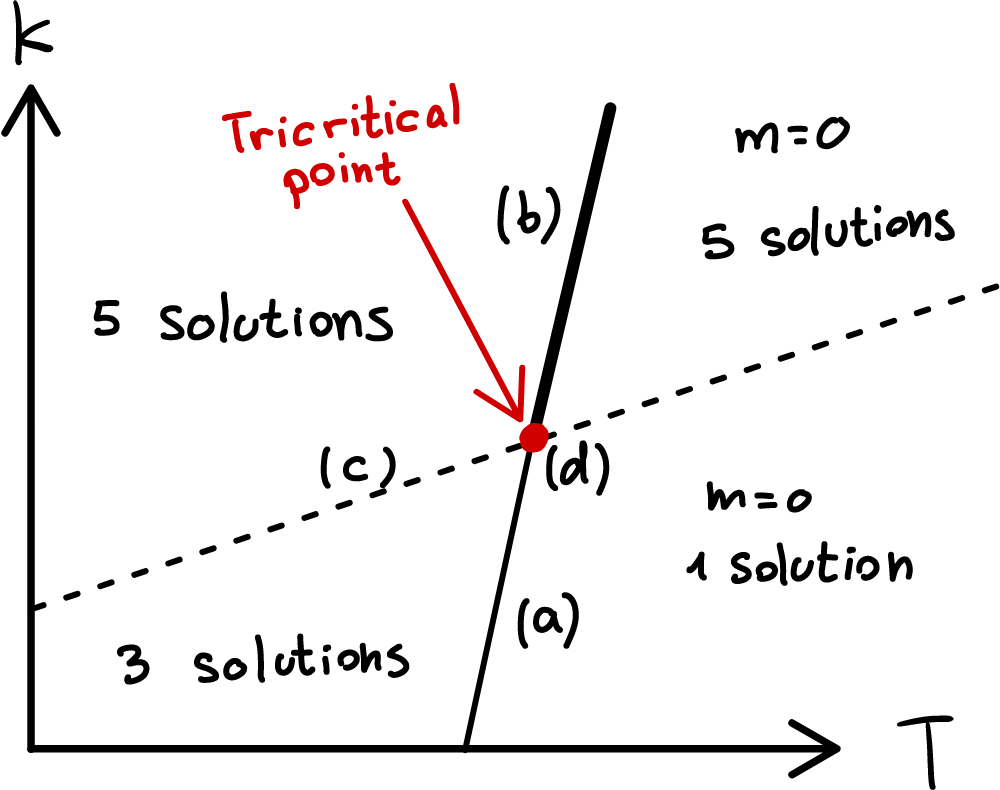
\includegraphics[width=0.5\textwidth]{phase-diagram-kt.png}
    \caption{The phase diagram of the model in the $K-T$ space. (a) The second order phase transition line, (b) the first order phase transition line, (c) the line seperating the 3-solutions and 5-solutions areas (d) the tricritical point}
    \label{fig:phase_diagram}
\end{figure}
\subsection{The Landau free energy}
The Landau free energy can be seen in figure \ref{fig:landau_free_energy} at different parts of the phase space.
\begin{figure}[h]
    \centering
    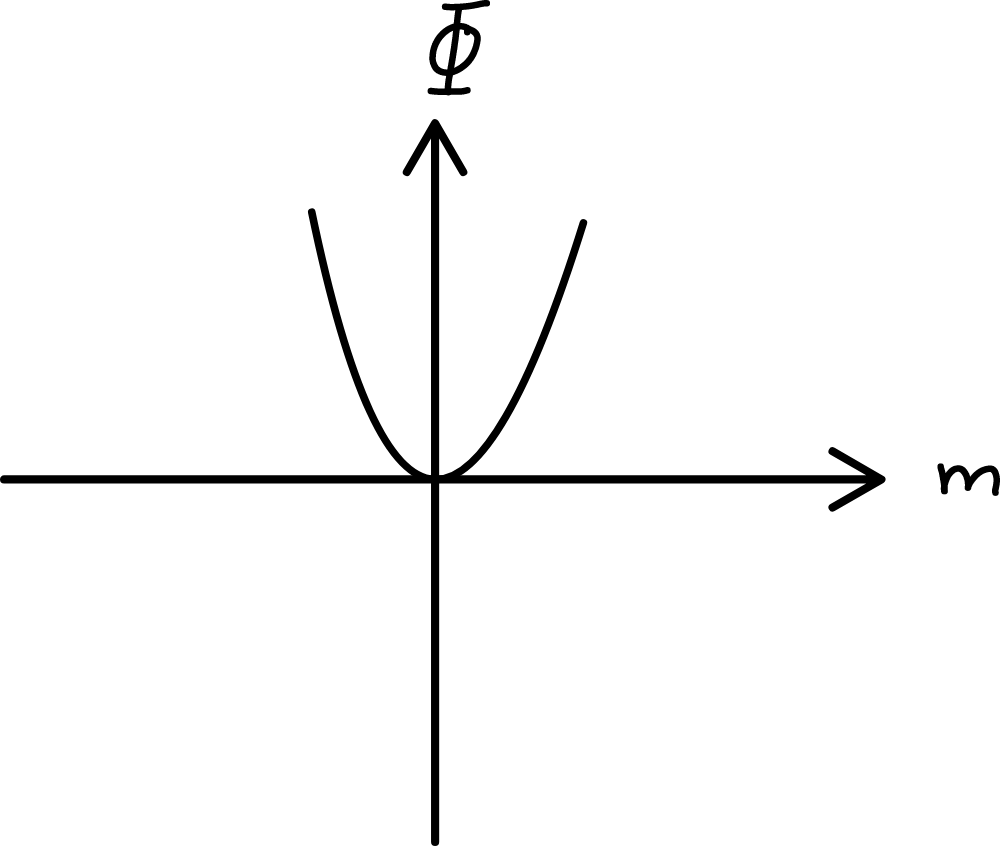
\includegraphics[width=0.3\textwidth]{phi-1.png}
    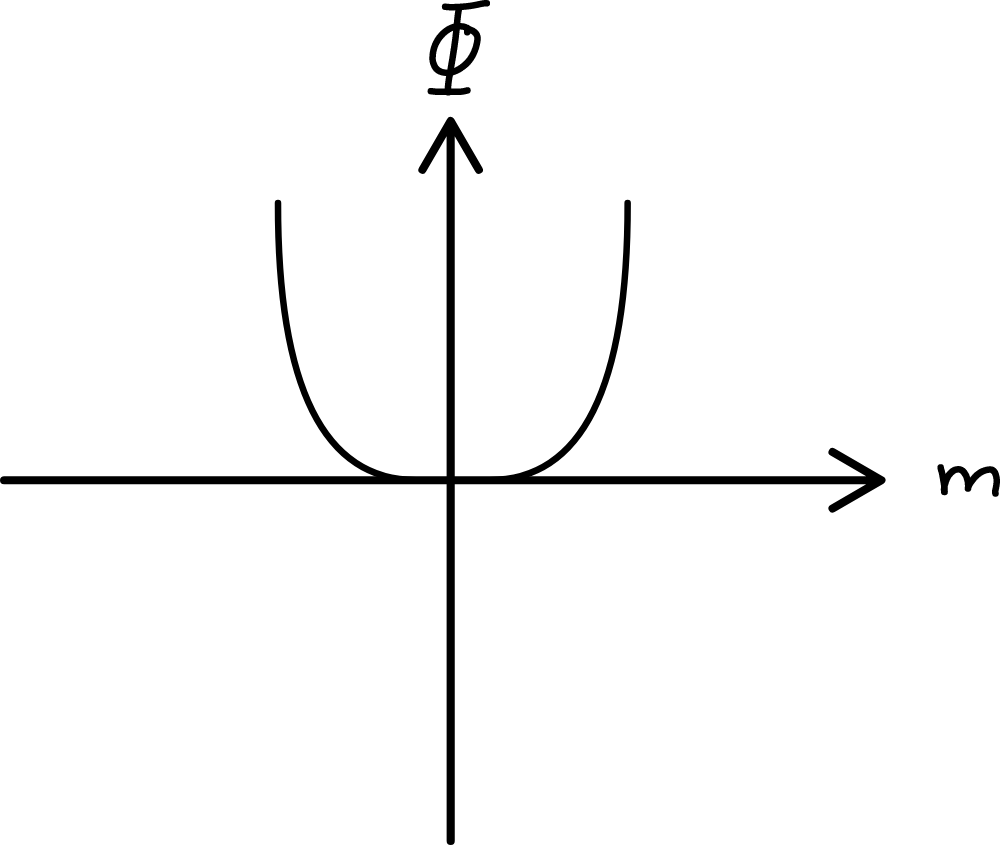
\includegraphics[width=0.3\textwidth]{phi-3-transition.png}
    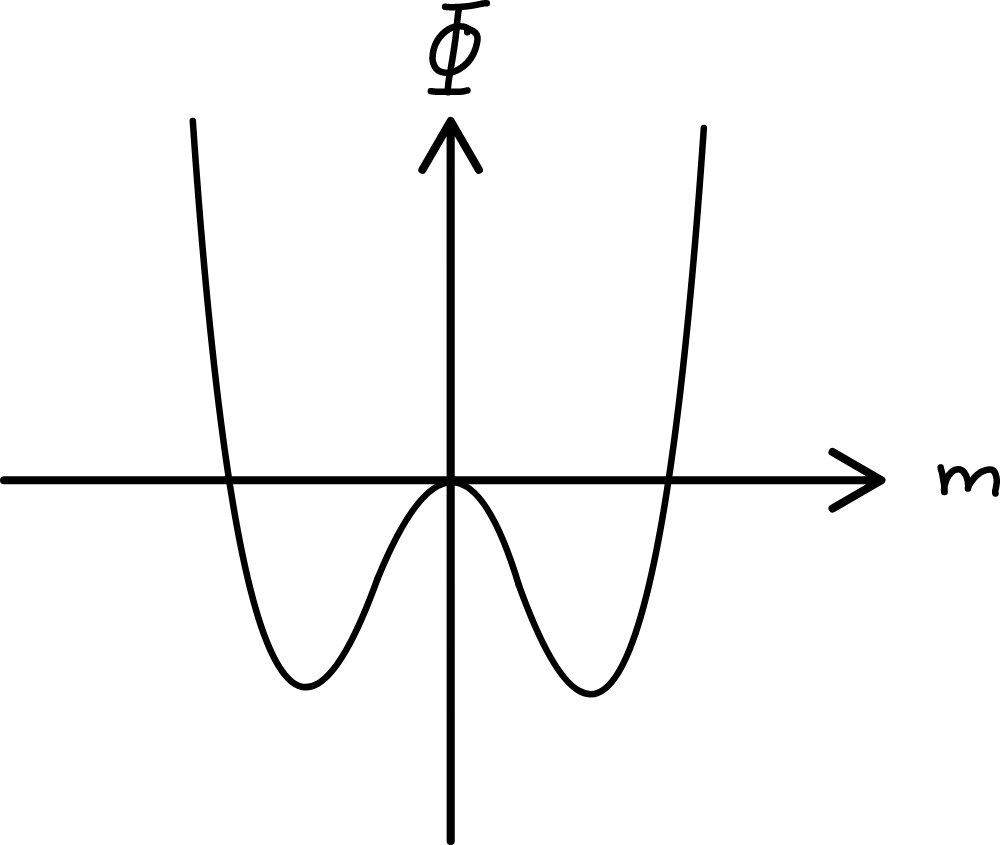
\includegraphics[width=0.3\textwidth]{phi-3-stable.png}
    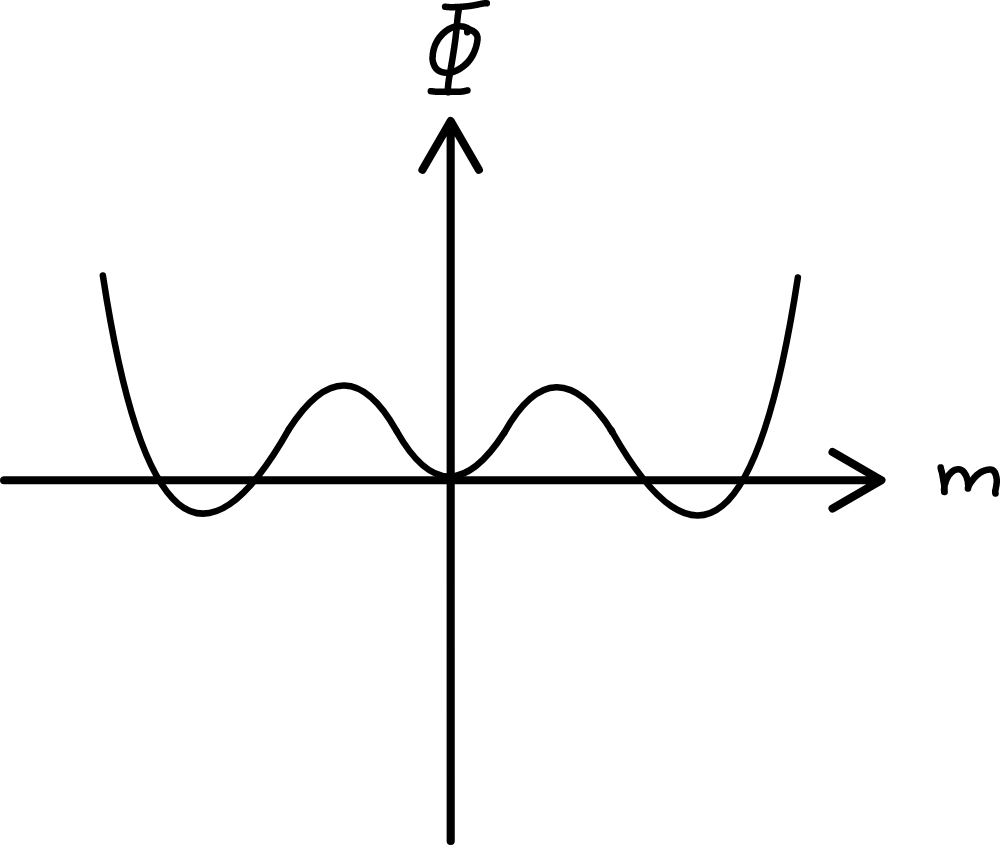
\includegraphics[width=0.3\textwidth]{phi-5-stable.png}
    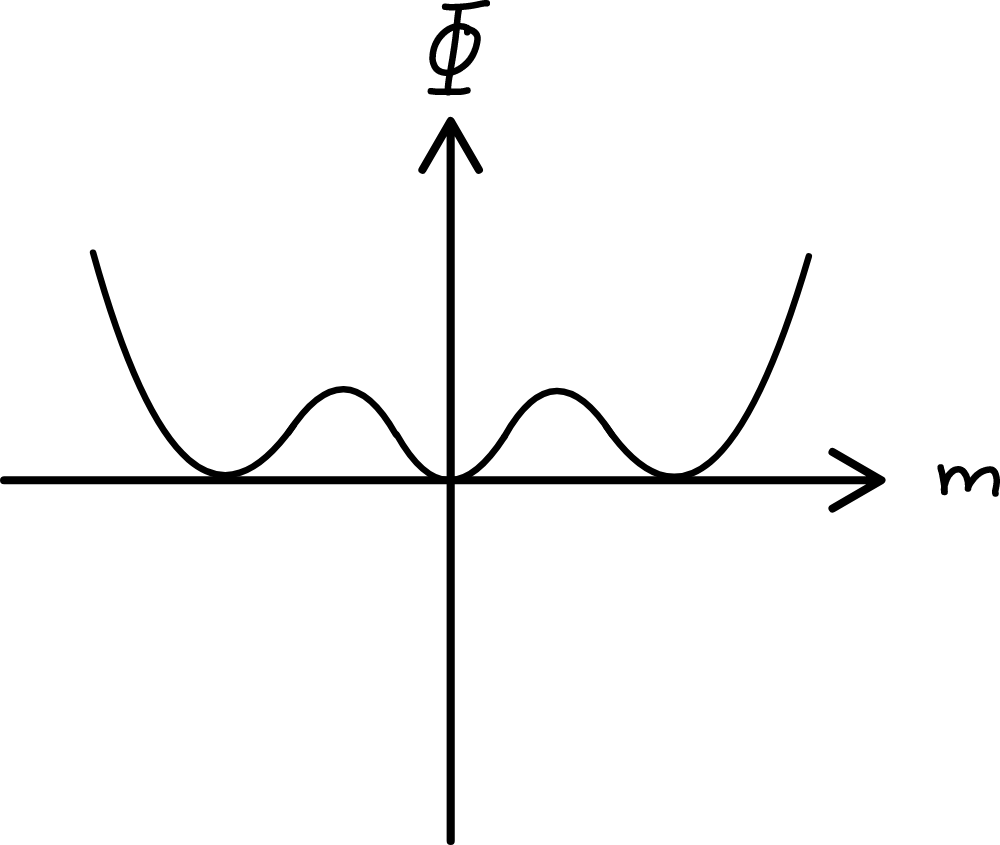
\includegraphics[width=0.3\textwidth]{phi-5-transition.png}
    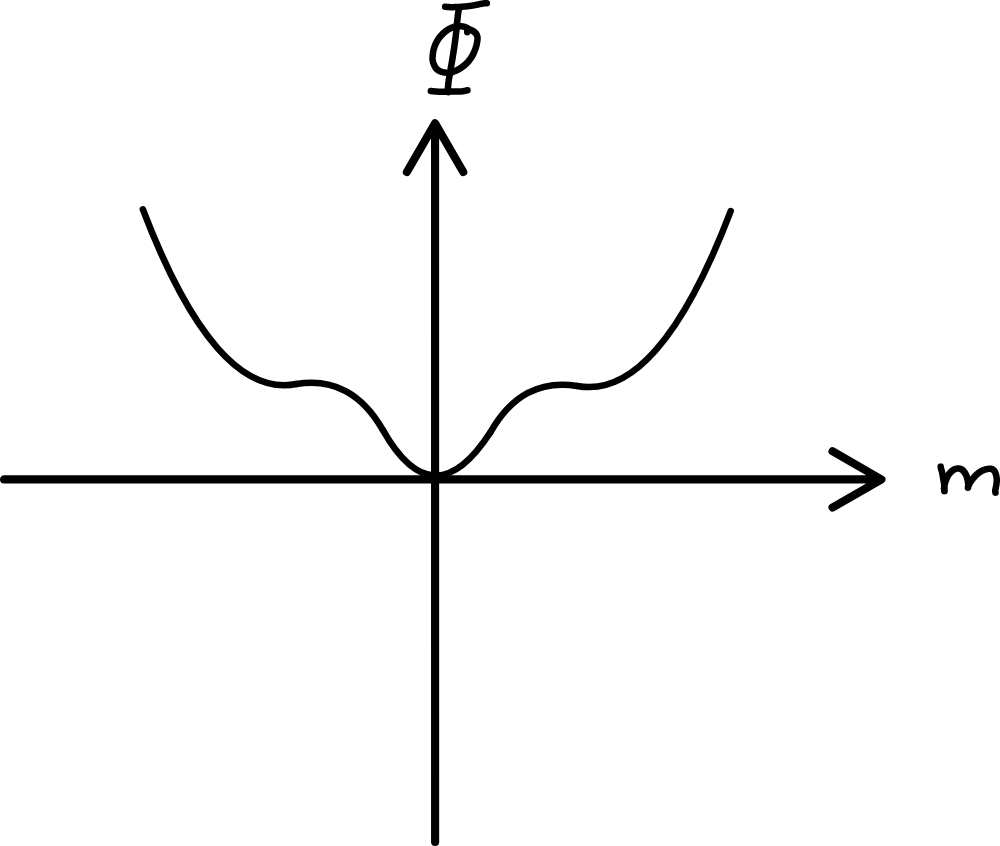
\includegraphics[width=0.3\textwidth]{phi-3-to-5-transition.png}
    \caption{The Landau free energy at different parts of the phase space. Top row: (left) unordered phase with one minimum at $m = 0$ (middle) at the second order phase transition point (right) ordered phase with two minima at $m \ne 0$. Bottom row: (left) ordered phase with two minima at $m \ne 0$ (middle) at the first order phase transition point (right) at the line seperating the 3-solutions and 5-solutions areas.}
    \label{fig:landau_free_energy}
\end{figure}
As can be seen, at some parts of the phase sapce the free energy has five extrema. This is possible only for a polynomial with degree six or above. Since for $h = 0$ the model retains the $m \rightarrow -m$ symmetry, the polynomial has only even powers except for the linear term with prefactor $h$, leading to the final form of the free energy:
\begin{equation}
    \Phi = -hm + am^2 + bm^4 + dm^6
\end{equation}
\subsection{Critical exponents}
Let us calcualte the critical exponents $\alpha$ and $\beta$ near the tricritical point. At that point,  For these two exponents, we set $h = 0$ and derive to find the minimising magnetization:
\begin{equation}
    \frac{\partial \Phi}{\partial m} = 2am + 4bm^3 + 6dm^5 = 0
\end{equation}
\begin{equation}
    m = 0, m^2 = \frac{-b \pm \sqrt{b^2 - 3ad}}{3d}
\end{equation}
At the tricritical point, all solutions converge, which requires $a = b = 0$. So, going along the line $d = const$ we can expand $a$ and $b$ as a function of $t = \frac{T - T_C}{T_C}$ and $k = \frac{K - K_C}{K_C}$ and keep only the first order. We care about the relation to $t$, so for small $t$, the smaller power is more significant, which is in this case the power of $a$ which is $1/4$, giving $\beta = 1/4$:
\begin{equation}
    m \sim \sqrt{\frac{-b \pm \sqrt{b^2 - 3ad}}{3d}} \sim \sqrt{\frac{-b_T t \pm \sqrt{b_T^2t^2 - 3d a_Tt}}{3d}} \sim t^{1/4}
\end{equation}
Now let us find $\alpha$ - the critical exponent of the heat capacity. For this, let us remember that the heat capacity can be calcualted from the free energy using:
\begin{equation}
    C = -\frac{\partial^2 F}{\partial T^2}
\end{equation}
The free energy is
\begin{equation}
    F = V\Phi(m_0, h = 0) = V(am^2 + bm^4 + dm^6)
\end{equation}
Since $a, b \sim t$ and $m \sim t^{1/4}$, we get:
\begin{equation}
    F \sim (t^{3/2} + t^{2} + t^{3/2}) \sim t^{3/2}
\end{equation}
\begin{equation}
    C \sim t^{-1/2}
\end{equation}
So we got $\alpha = 1/2$. Unsurprisingly, we got different critical exponents from the Ising model.

\newpage
\section{Landau Theory for the XY model}
Let us consider the XY model:
\begin{equation}
    H = \sum_{\langle i, j \rangle} \vec{S}_i \cdot \vec{S}_j - \vec{B} \sum{i} \vec{S}_i
\end{equation}
where $S_i = \left(\cos\theta_i, \sin\theta_i\right)$ for some real $\theta_i$.
\subsection{The Landau Free Energy}
In this model, we can define an order parameter $\bar{S}$ which is the average spin configuration over an area. For an external field $B = 0$, there is a rotation symmetry $O(2)$, which means only the size of $\bar{S}$ matters, i.e. we get only even terms in $\bar{S}$. When $B \ne 0$, we get an additional $\vec{B}\cdot\bar{S}$ linear term:
\begin{equation}
    \Phi(\bar{S}, T, B) = -\vec{B}\cdot\bar{S} + aS^2 + bS^4
\end{equation}
\subsection{Critical Exponents}
Let us now calculate the critical exponents $\alpha, \beta, \gamma,$ and $\delta$. At $B = 0$:
\begin{equation}
    \Phi(\bar{S}, T, B) = aS^2 + bS^4
\end{equation}
This is very similar to the Ising model with $S$ instead of $m$, and so we expect the exponents to be the same. So, looking at $b > 0$, since that is where the system has minima, we get:
\begin{equation}
    S_0^2 = \begin{cases}
        \pm \frac{a}{2b} & a < 0 \\
        0 & a > 0
    \end{cases}
\end{equation}
Which means $a$ acts like $t = \frac{T - T_c}{T_c}$. On the other hand, $b$ must be greater then zero, and so it has a zeroth order. So, around $t = 0 \rightarrow a = 0$, in leading order:
\begin{equation}
    a \approx a_0 (T - T_c)
    \qquad
    b \approx b_0
\end{equation}
This gives:
\begin{equation}
    S_0 = \sqrt{\frac{2a}{b}} \approx \sqrt{\frac{a_0T_c t}{2b_0}} \sim t^{1/2}
\end{equation}
So the first cirtical exponent is $\beta = 1/2$. Next, let us look at the susceptibility $\chi$ at $T > T_c$. For this, we go back to $B \ne 0$, and keeping again the first two terms, we can set $b = 0$. In this case:
\begin{equation}
    \bar{S}_0 = \frac{1}{2a}\vec{B} \approx \frac{1}{2a_0T_c t}\vec{B}
\end{equation}
And so
\begin{equation}
    \chi = \nabla_{B}\bar{S} = \frac{1}{2a_0T_c t} \sim t^{-1}
\end{equation}
Which gives, as expected $\gamma = 1$. Next let us calcualte $\alpha$. The free energy is given by
\begin{equation}
    F = V \Phi(S_0, B=0) = V\left(\pm \frac{2a^2}{b} + \frac{4a^2}{b}\right) \sim V\frac{a^2}{b} \sim t^2
\end{equation}
So
\begin{equation}
    C \sim const
\end{equation}
And we got the expected $\alpha = 0$. Finally, let us look at $\delta$, which encodes the ratio of $\bar{S}$ and $\vec{B}$ at the cirtical point, rather then above it like $\gamma$. For this, let us take the model at $t = 0$ and $B \ne 0$. This means, since $a \sim t = 0$, we get:
\begin{equation}
    \Phi \sim -\vec{B}\cdot\bar{S} + b_0S^4 = -\vec{B}\cdot\bar{S} + b_0S^2(\bar{S}\cdot\bar{S}) = \left(-\vec{B} + b_0S^2\bar{S}\right)\cdot\bar{S}
\end{equation}
\begin{equation}
    \nabla_S \Phi = -\vec{B} + b_0S^2\bar{S} = 0
\end{equation}
\begin{equation}
    \bar{S}_0 = \left(\frac{|\vec{B}|}{b_0}\right)^{1/3}\hat{B}
\end{equation}
Which gives $\delta = 1/3$.
\subsection{The susceptibility prefactor ratio}
Let us look at the prefactors of the susceptibility above and below the critical point. We calcaulted $\chi_{+}$ in the previous section, let us now calculate $\chi_{-}$ for $t < 0$. This time, since it takes part of the minimization, we cannot ignore $b$. For this, let us take $S_0$ to be the minimum $S_0^2 = \pm \frac{2a}{m}$ and expand around it $\bar{S} = \bar{S}_0 + \delta\bar{S}$ where $\delta\bar{S}$ encodes the effects of $\vec{B}$. This gives
\begin{equation}
    \Phi = - \vec{B}\cdot\delta\bar{S} +
    a\delta S^2 + 2a \bar{S}_0 \cdot \delta\bar{S} +
    b\delta S^4 + 4b \delta S^2 \delta\bar{S} \cdot \bar{S}_0 +
    2b \delta S^2 S_0^2 + 4b\left(\bar{S}_0 \cdot \delta\bar{S}\right)^2 +
    4b S_0^2 \bar{S}_0 \cdot \delta\bar{S}
    + f(S_0)
\end{equation}
Where $f(\bar{S}_0)$ encodes all the information about $\bar{S}_0$ that we do not care about, since we are about to derive by $\delta \bar{S}$. Grouping the terms by order in $\delta S$:
\begin{equation}
    \Phi = b\delta S^4
    + 4b \delta S^2 \delta\bar{S} \cdot \bar{S}_0
    + (a + 2b S_0^2) \delta S^2 + 4b\left(\bar{S}_0 \cdot \delta\bar{S}\right)^2
    - \vec{B}\cdot\delta\bar{S}
    + \left(2a \bar{S}_0 + 4 b S_0^2 \bar{S}_0\right) \cdot \delta\bar{S}
    + f(S_0)
\end{equation}
Since by the definition of $\bar{S}_0$
\begin{equation}
    2a \bar{S}_0 + 4 b S_0^2 \bar{S}_0 = 2(a + 2 b S_0^2) \bar{S}_0 = 0 
    \rightarrow
    a + 2 b S_0^2 = 0
\end{equation}
so the first square term and the second linear term vanish. Keeping only up to second order in $\delta \bar{S}$, we get:
\begin{equation}
    \Phi = 4b\left(\bar{S}_0 \cdot \delta\bar{S}\right)^2
    - \vec{B}\cdot\delta\bar{S}
    + f(S_0)
\end{equation}
Deriving by $\delta \bar{S}$ we get:
\begin{equation}
    \nabla_{\delta S} \Phi = 8b\left(\bar{S}_0 \cdot \delta\bar{S}\right) \bar{S}_0 - \vec{B} = 0
\end{equation}
Which is solved by:
\begin{equation}
    \delta \bar{S} = \frac{1}{8bS_0^2}\vec{B} = \frac{1}{4a_0}\vec{B}
\end{equation}
And so we get $A_{+} = \frac{1}{2a_0}$ and $A_{-} = \frac{1}{4a_0}$ so the ratio $A_{+} / A_{-} = 2$ matches the ratio we found for the Ising model.
\end{document}